\documentclass[11pt]{article}
\usepackage[utf8]{inputenc}

\usepackage{amssymb, amsmath, amsthm, amsfonts, algorithmic, algorithm, graphicx}
\usepackage{color}
\usepackage{bbm}
\usepackage[dvipsnames]{xcolor} 
\usepackage[colorlinks,linkcolor=blue,citecolor=blue]{hyperref}
\usepackage{array}
\usepackage{ifthen}
\usepackage{subfigure}
\renewcommand{\baselinestretch}{1.1}
\setlength{\topmargin}{-3pc}
\setlength{\textheight}{8.5in}
\setlength{\oddsidemargin}{0pc}
\setlength{\evensidemargin}{0pc}
\setlength{\textwidth}{6.5in}

\newtheorem{theorem}{Theorem}[section]
\newtheorem{lemma}[theorem]{Lemma}
\newtheorem{proposition}[theorem]{Proposition}
\newtheorem{corollary}[theorem]{Corollary}
\newtheorem{question}[theorem]{Question}
\newtheorem{result}[theorem]{Result}
\newtheorem{definition}[theorem]{Definition}
\newtheorem{example}[theorem]{Example}
\newtheorem{remark}[theorem]{Remark}
\newtheorem{assumption}[theorem]{Assumption}
\numberwithin{equation}{section}

\def \endprf{\hfill {\vrule height6pt width6pt depth0pt}\medskip}
\renewenvironment{proof}{\noindent {\bf Proof} }{\endprf\par}

% Notational convenience,
% real numbers 
\newcommand{\R}{\mathbb{R}}  
% Expectation operator
\DeclareMathOperator*{\E}{\mathbb{E}}
% Probability operator
\DeclareMathOperator*{\Prob}{\mathbb{P}}
\renewcommand{\Pr}{\Prob}

% You may define additional macros here.


\begin{document}

\begin{center}
    \sc Recurrent and Generative ANNs
\end{center}

\noindent Name: Bileam Scheuvens, Pankaj Bora

\noindent Email: benedictbileam@gmx.de, bora.pankajt1@gmail.com

\noindent Matr. Nr.:6983475, 6946375



\section*{Exercise 1}
\subsection*{(a,b,c,d)}
Memory Task:


LSTM and RNN achieve perfect predictions, but LSTM show smoother convergence than RNNs


TCN converges significantly quicker than both but fails to predict perfectly, maybe due to struggling with positional dependencies
\newline
\newline
MemoryGen Task:


RNN generalizes better with lower validation loss and perfect predictions for the examples


LSTM also has prefect predictions but suffers with instability in validation loss, so it doesn't generalize as well to shifted token positions


TCN generalizes and converges very rapidly initially but overfits over time and produces slightly inaccurate predections

\newline

\begin{figure}[H]
  \centering % Centers the image
  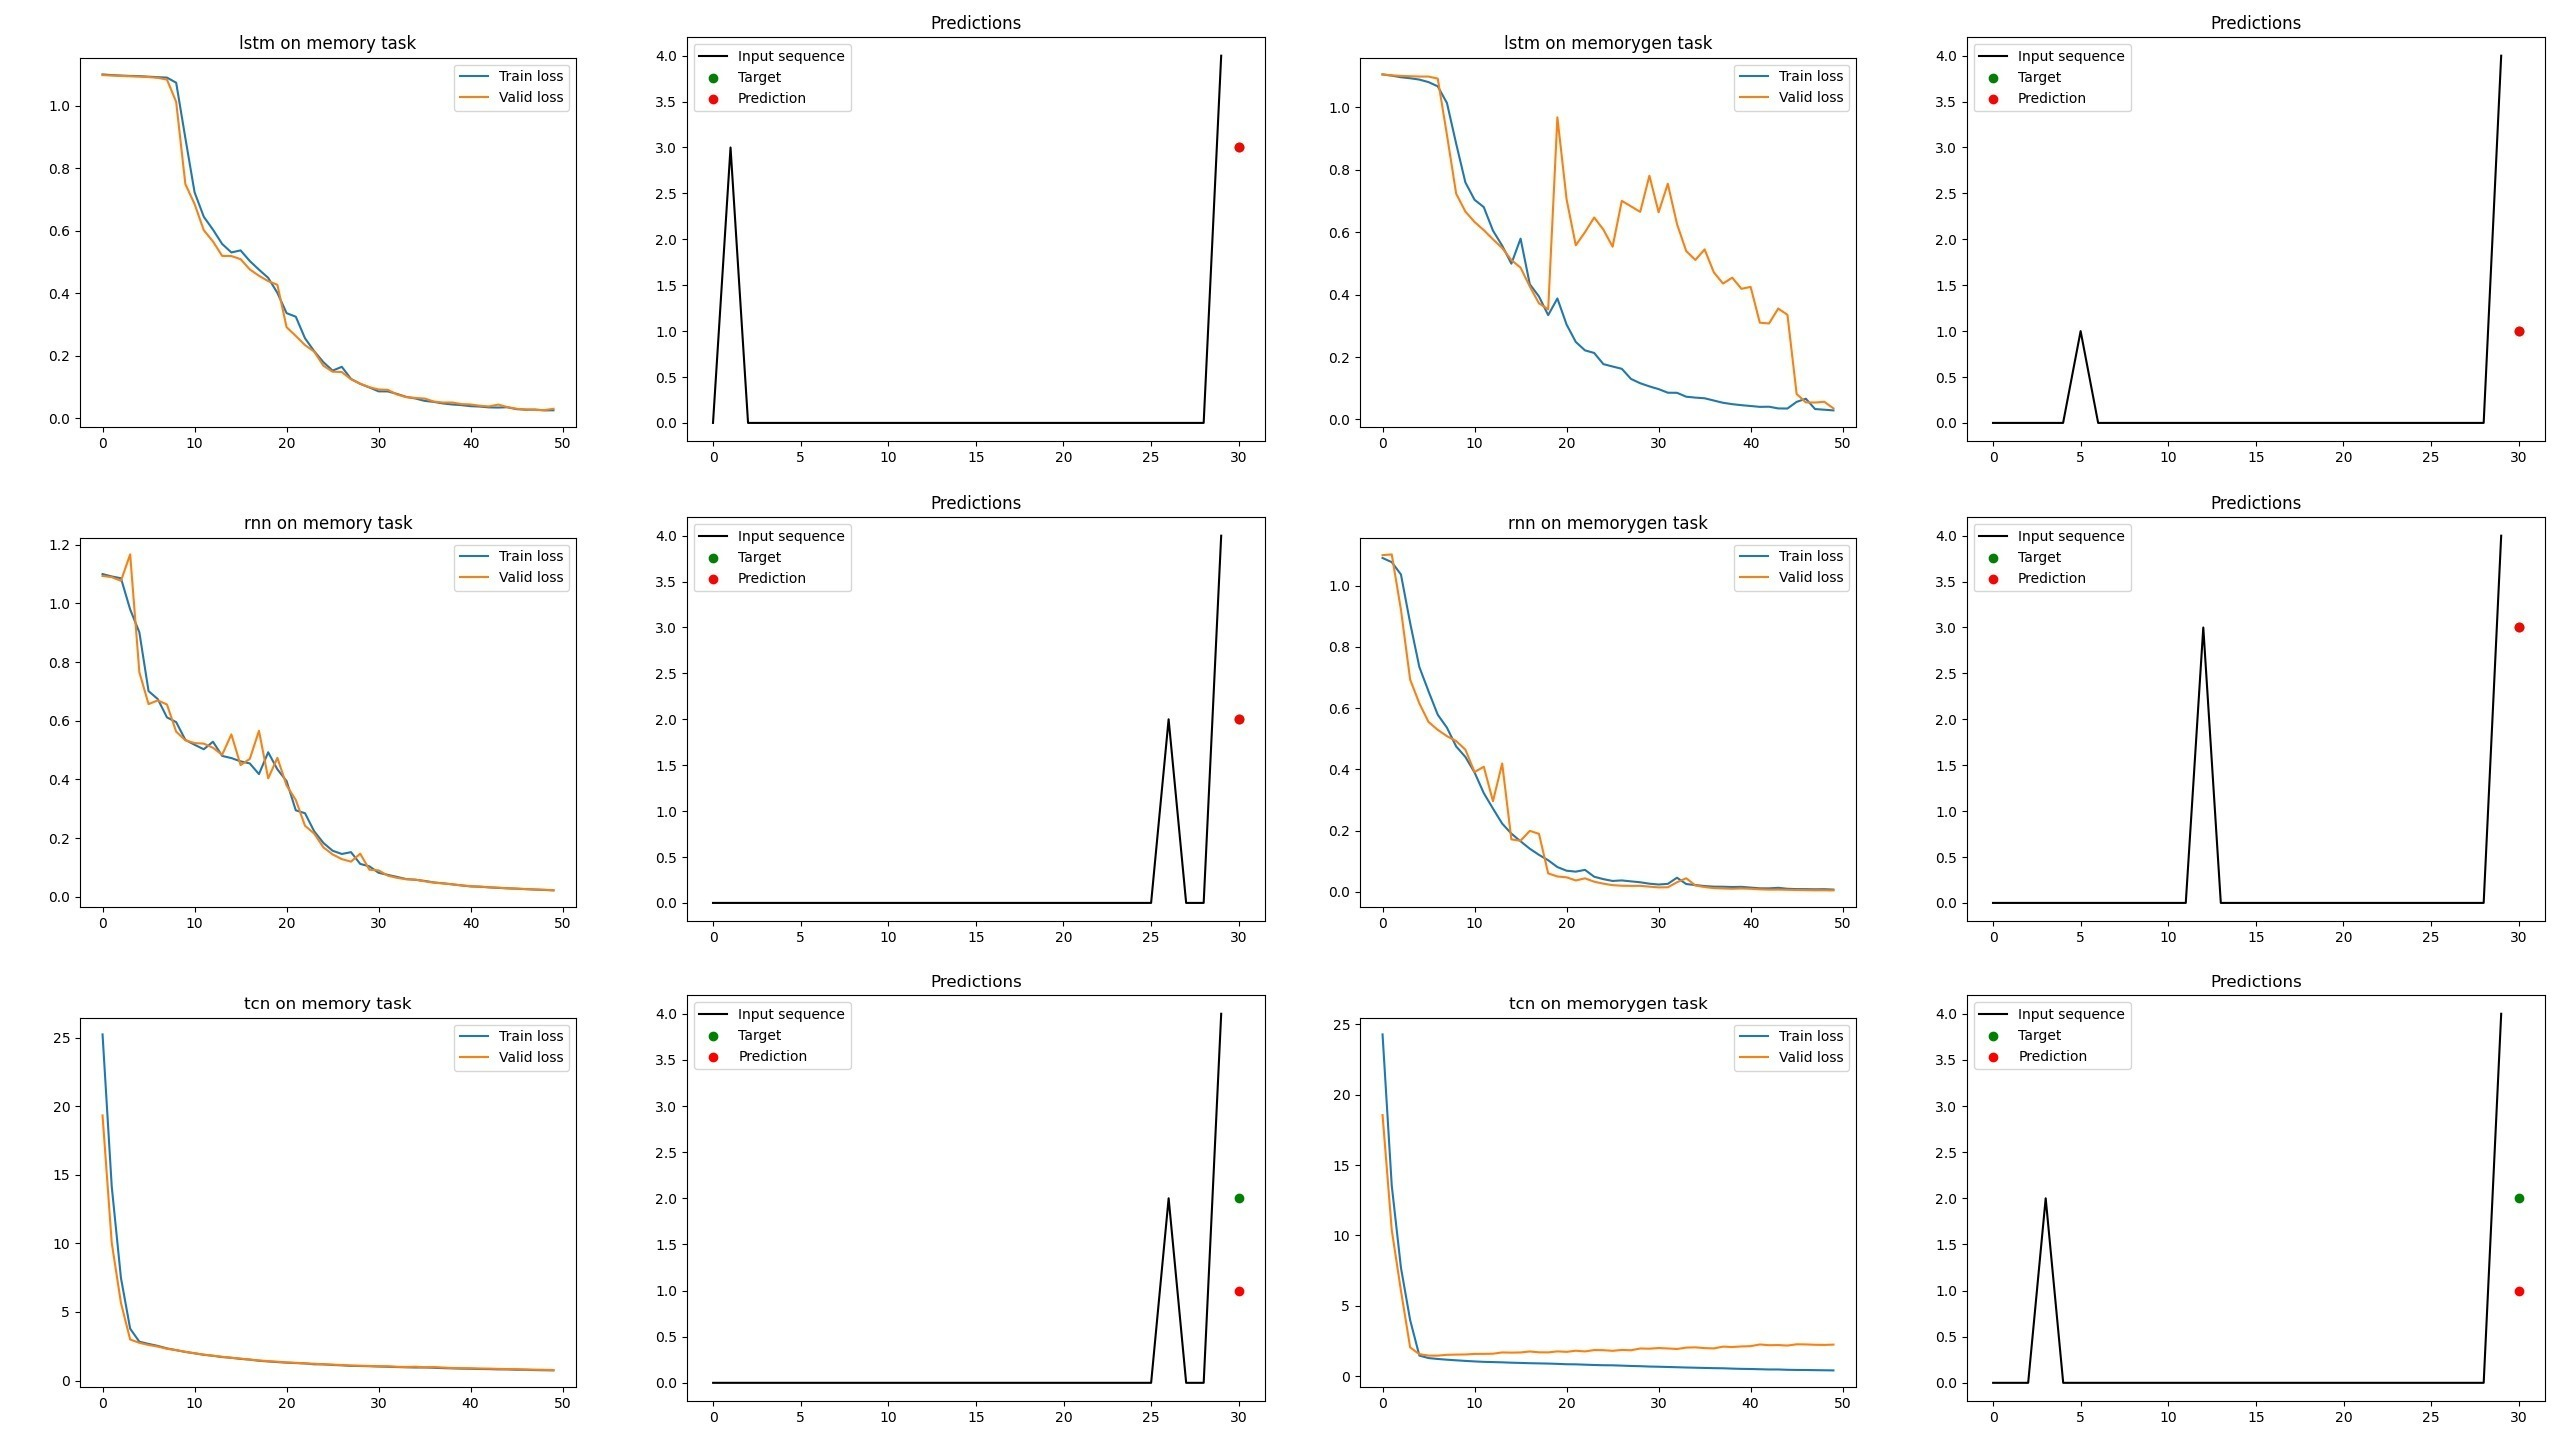
\includegraphics[width=1.1\textwidth]{imageAll.jpg} % Adjust width as needed
\end{figure}


\section*{Exercise 2}
\subsection*{(a,b)}
See code for implementation.

\subsection*{(c)}
The model performs well for all static or consistently changing environments, such as the trees, the path or the player when standing still.
Since inputs are not available to the model, it cannot predict the player's movement leaving it to be very unsure of player position and completely dropping the sprite after just a few frames.

\subsection*{(d)}
Without attention the model has no concept of spatial relationships between patches, it merely learns that the player is at the center of the image and outputs this as a static prediction. Attention helps put individual activations into context, which is necessary to understand surrounding.

\subsection*{(e)}
Without positional embeddings the model performs very poorly and converges to point of treating all patches equally. The output is a homogenous blur resembling the texture of what could be a tree.

\subsection*{f}
Without a thorough gridsearch we found it difficult to make definite conclusions about the architecture. Since jobs on the cluster are strictly time limited, more than limited exploration of the search space was not possible.
More complexity(n\_layers / heads) seemed to be beneficial, as well a larger learning rate. Increasing the number of frames in the input sequence slowed down convergence, it is unclear if the final performance would be better since the model was not able to converge within the time limit.
The same can be said for increasing the model complexity drastically.
The patch size seemed optimal at 16x16, as 32x32 does not divide the image evenly and 8x8 or 4x4 increase memory demands and slow down convergence significantly in terms of time, while being more sample efficient.
Weight decay, mixed precision and gradient\_accumulation\_steps were not explored.
Batch size was fixed as the scaling laws dictate the ratio to the learning rate, which was optimized.

For the final configuration we obtain the default configuration with the following adjustments:
"num\_heads": 4
\newline
"layers": 6
\end{document}
